\documentclass[12pt]{article}
\usepackage{fullpage}
\usepackage[margin=1in]{geometry}
\usepackage[stable]{footmisc}
\usepackage{graphicx}
\usepackage{amssymb}
\usepackage{IEEEtrantools}
\usepackage{lineno}
\usepackage{amsmath}
\usepackage{epstopdf}
\usepackage{parskip}
\usepackage{authblk}
\usepackage[authoryear]{natbib}
%\setlength{\parskip}{20pt}
\linespread{1.6}
\date{}

\DeclareGraphicsRule{.tif}{png}{.png}{`convert #1 `dirname #1`/`basename #1 .tif`.png}


%%	math short-cuts
\def \ve{\varepsilon}	% epsilon used for metabolic rate
\def \la{\lambda}	% lambda
\newcommand{\eref}[1]{( {#1})}

%%	new commands for referencing figures and tables and sections
\newcommand{\fref}[1]{Figure~\ref{#1}}	% inline figure ref
\newcommand{\fpref}[1]{Fig.~\ref{#1}}	% parenthetical figure ref
\newcommand{\tref}[1]{Table~\ref{#1}}	% table ref
\newcommand{\sref}[1]{Section~\ref{#1}}	% table ref
%\linenumbers

\title{\Large \textbf{Generating oscillations in MERA: differentiate generation time from allocation period}}

\author{Jade, Nov 16}

\begin{document}
\maketitle
\raggedright
\large
\setlength{\parindent}{15pt}

From results in the previous write-ups we can see that, under the current framework of MERA, for both the single species case and the multiple competitors case, population size does not oscillate even when the intrinsic growth rate $r$ is very high (as opposed to the predictions of the logistic growth equation and the Lotka Volterra equations). Through time, each species converges smoothly to its steady state and stays there once steady state is reached. 

In this write-up I will first explore the temporal assumptions of MERA compared to other models to infer which part possibly eliminates oscillations. Next I will prove that the relaxing of this assumption does generate oscillations under the MERA framework. The conclusion is that the difference between generation time and allocation period is probably at the root of population oscillations.

\section{A projection: oscillation, discretion and time lag}

We all know that the discrete logistic growth equation leads to oscillations around the steady state when intrinsic growth rate is high, while its continuous counterpart does not. One way to look at this is that, in the discrete logistic growth model, there is a time lag (the length of $\Delta t$) for the population to react to the density dependence effects imposed by its abundance. During this lag period, population size and density dependence information is not updated and the population grows at the same speed as at the beginning of the period, creating a chance for over shooting. In the continuous model, however, there is no time lag and density dependence information is instantly updated, therefore the population can adjust its growth rate instantly in response to its size at every moment, leaving no chance for over shooting. 

Now let's look at MERA. In MERA, the form of density dependence is realized through the resource allocation process. So far we have assumed that the generation time is the same as the resource allocation period, therefore the population size updates every time (and only when) resource is allocated. This means that every time the form of density dependence changes, the population instantly reacts to it, or there is no time lag for the population to react to the density dependence effects imposed by its abundance. Therefore, although MERA is seemingly a discrete model (since resource allocation happens in discrete time steps), by the criteria described above, it actually more closely models continuous growth since there is no time lag for population growth rate to react to its abundance, which is probably the reason why we do not see oscillations in MERA predictions. 

So far it has been my projections and some of the arguments might be invalid or need re-wording. However, it is easy to test the resulting inference: if we introduce time lag into MERA, i.e. population size does not change every time resource is allocated and resource needs to be accumulated for several allocation periods (corresponding to one generation time) before population size can be updated, a different dynamic pattern (possibly with oscillations) is expected. Since generation time is species specific in nature, this is a particularly important assumption to explore for both the single species case and multiple species cases where generation time not only differs from allocation period, but also potentially varies among species.

\section{Introducing species specific generation time into MERA}

To relax the previous assumption of species generation time is the same with resource allocation period, here an extra parameter $G_i$ is introduced to represent the generation time for species $i$, or the number of allocation periods resource has to be accumulated before the population size of species $i$ changes. It is assumed to be a positive integer greater than or equal to 1 ($G_i \geq 1$), which is of course an approximation of reality but should be accurate enough especially when resource allocation period is much smaller than the generation time. Although complications in real world could generate violations of these assumptions, I think it is OK to bear with them to take a first look at the effect of $G_i$.

\subsection{Single species case: increased oscillations with $D_r$ and $r$}

The previous single species model is equivalent to $G_1=1$, or growth is only accumulated for one allocation period before added on to the population. This leads no oscillations under all conditions (Fig.1).

\begin{figure}
 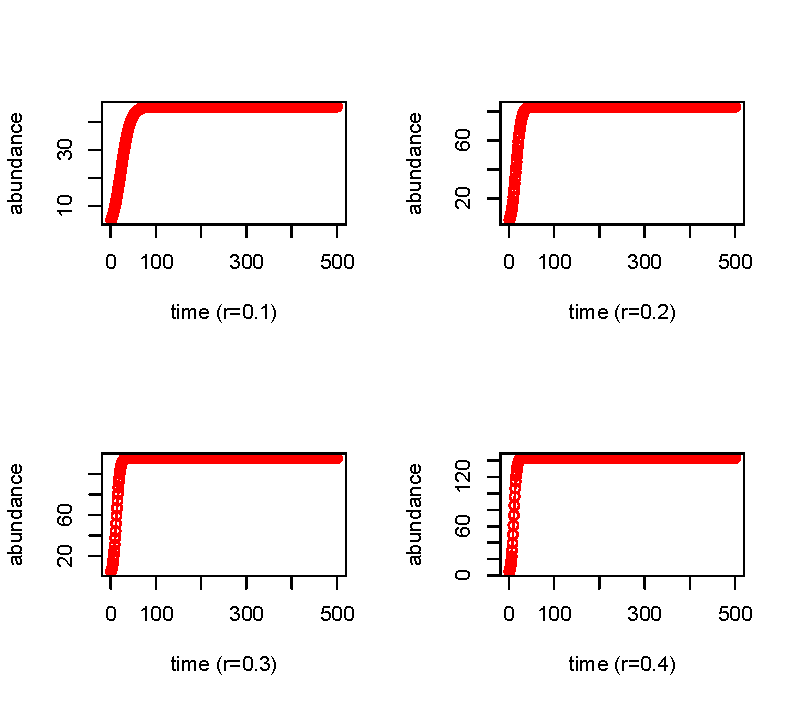
\includegraphics[width=\textwidth]{1sp_no_sojourn.pdf}
 \caption{Single species growth with no time lag ($G_1=1$)}
For all four graphs $ N_{1,t=0}=5, \theta_1=1, D_{r,1} = 0, R_0=500$. The value of $r$ is shown under the x-axis.
\end{figure}

Now let's look at the case where $G_1=10$, so that generation time is ten times as long as one allocation period, or growth (positive or negative) has to be accumulated for 10 allocation periods before added on to the population (Fig. 2 \& 3).

\begin{figure}
 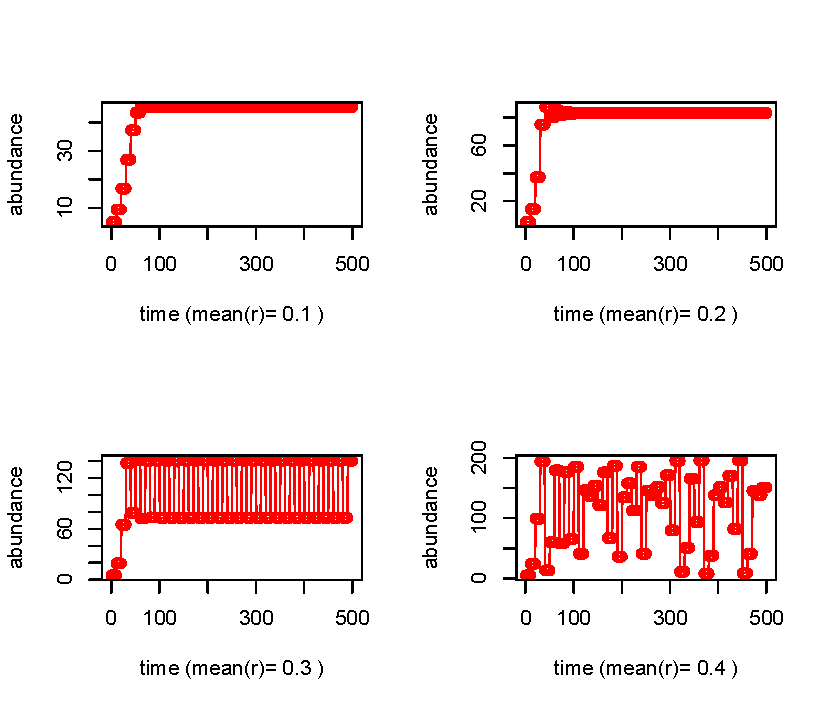
\includegraphics[width=\textwidth]{1sp_sojourn.pdf}
 \caption{Single species growth with time lag ($G_1=10$)}
For all four graphs $ N_{1,t=0}=5, \theta_1=1, D_{r,1} = 0, R_0=500$. The value of $r$ is shown under the x-axis.
\end{figure}

\begin{figure}
 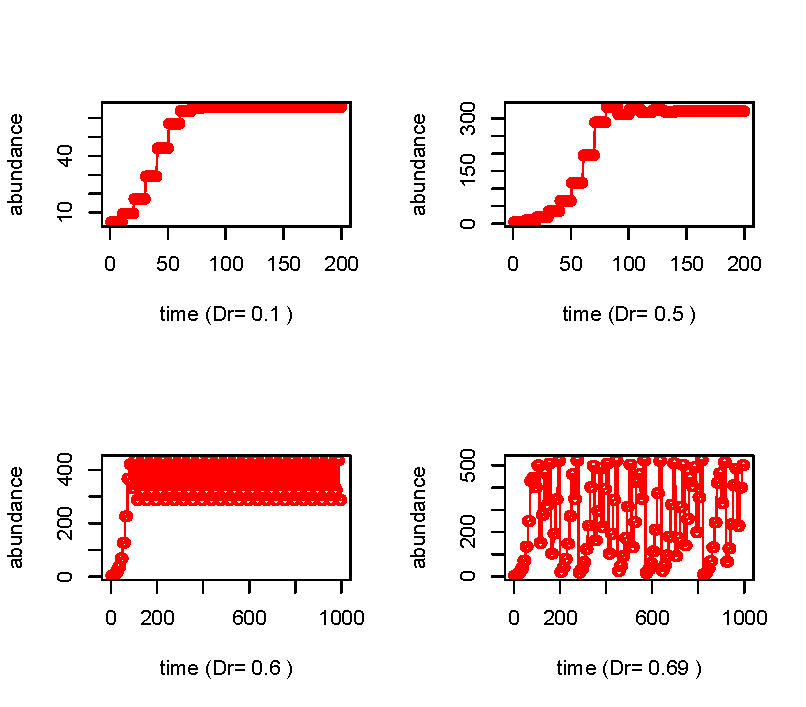
\includegraphics[width=\textwidth]{1sp_sojourn_Dreffect.pdf}
 \caption{$D_r$ effect on single species growth with time lag ($G_1=10$)}
For all four graphs $ N_{1,t=0}=5, \theta_1=1, r_1= 0.1, R_0=500$. The value of $D_{r,1}$ is shown under the x-axis.
\end{figure}

From Fig. 2 and Fig. 3 we can see that, when the species generation time is not the same as the resource allocation period, all else equal, the bigger the $r$ or the bigger the $D_r$, the more oscillations in population dynamics. Actually when you look across the graphs in each figure, you'll see that the effect of increasing $r$ and $D_r$ is very similar to that of the intrinsic growth rate in the logistic growth function. 

\subsection{Multiple competitors case: differential generation time among species}
\begin{figure}
 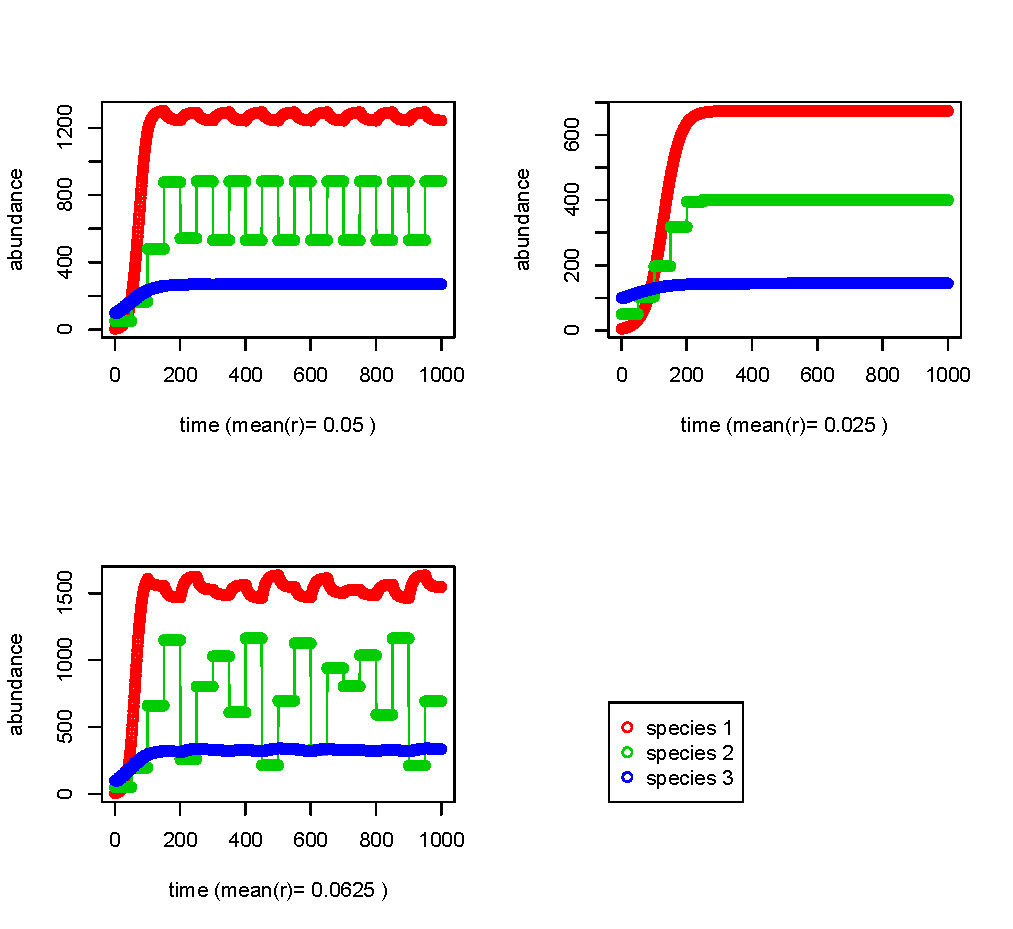
\includegraphics[width=\textwidth]{oscillation_r_effect.pdf}
 \caption{Multiple species competing for one fundamental resource with differential generation time ($G_1=1, G_2=50, G_3=10$)}
For all four graphs $ N_{1,t=0}=5, N_{2,t=0}=50,N_{3,t=0}=100, D_{r,1}=D_{r,2}=D_{r,3}=0.1, \theta_1=\theta_2=\theta_3=1, r_1: r_2:r_3= 8:5:2, R_0=10000$. The mean value of $r$s is shown under the x-axis.
\end{figure}

\begin{figure}
 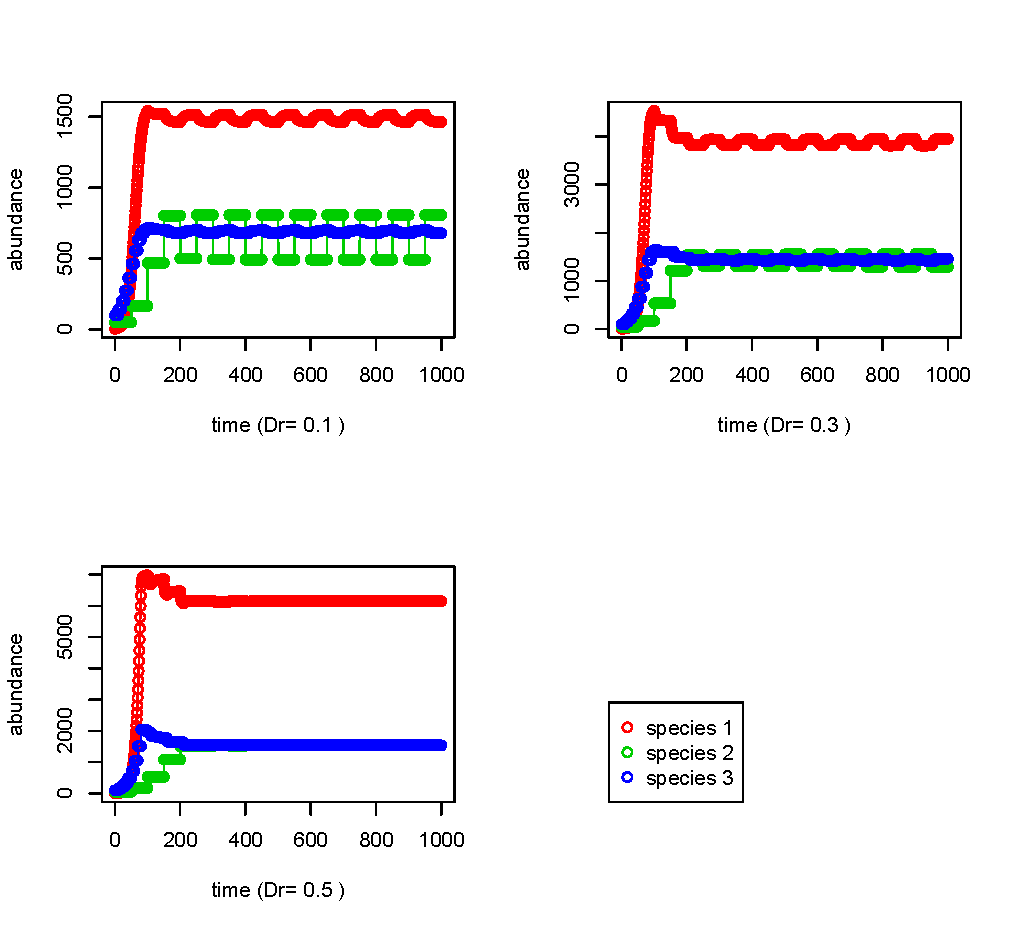
\includegraphics[width=\textwidth]{oscillation_Dreffect.pdf}
 \caption{$D_r$ effect on multiple species competing for one fundamental resource with differential generation time ($G_1=1, G_2=50, G_3=10$)}
For all four graphs $ N_{1,t=0}=5, N_{2,t=0}=50,N_{3,t=0}=100, \theta_1=\theta_2=\theta_3=1, r_1=0.08, r_2 =0.05, r_3= 0.02, R_0=10000$. $D_r$ is set to be the same for all species, the value is shown under the x-axis.
\end{figure}

From Fig. 4 and Fig. 5 we can see that, when there are species with generation time bigger than 1, populations for all species (including those with generation time equal to 1) oscillate. Fig. 4 shows that similar to the single species case, bigger $r$ for all species leads to more oscillations. However, Fig. 5 shows that bigger $D_r$ for all species leads to reduced oscillations, which is contrary to the single species case. This suggests that there is probably a tradeoff between intra- and interspecific competition in generating oscillations. In future analysis I will look into more parameter settings.

\section{Discussion: fitting the new model with allocation period and generation time}

In classic models they assume resource allocation is continuous. To compare with that, simply assume allocation period to be very small. Then $R_0$ and $\theta$ and $r$ are all very small.

 Then only one extra parameter: $G_i$. Previous clock is only in $r_i$, now in $G_i$ also. $R_0$ and $\theta$ only ratio matters.

Or fit one extra parameter, assuming resource allocation can be continuous or discrete.

Simulate with two models one with larger resource allocation period, the other with smaller allocation period (all else equal ratio dependent, bigger $G$ smaller $R_0$, $\theta$ and $r$) see if allocation period is trivial.

More important for predator-prey interactions



\end{document}